%---------------------------------------------------------------
\chapter{Testování}
\label{testovani}
%---------------------------------------------------------------

\begin{chapterabstract}
    V této kapitole otestuji naprogramovaný server, REST API a mobilní aplikaci pomocí automatizovaných a uživatelských testů. Následně opravím chyby, které zjistím v průběhu automatizovaných testů a zapracuji zpětnou vazbu z uživatelských testů.
\end{chapterabstract}

Po naprogramování první verze aplikace před jejím samotným vypuštěním na trh je vhodné aplikaci řádně otestovat. Existují dva základní typy testů, které lze použít k testování -- automatizované testy a uživatelské testy. Server, REST API i mobilní aplikaci jsem průběžně testoval pomocí automatizovaných i uživatelských testů.

\section{Automatizované testy}

Automatizované testy jsou takové, které programátor jednou napíše a spouští se automaticky, například při každém odeslání kódu do verzovacího systému. Jelikož jsou automatizované testy prováděny počítačem, jejich výsledkem je pouze úspěch/neúspěch, v případě neúspěchu pak většinou výpis očekávaný/skutečný výsledek. Velkou výhodou těchto testů je jejich automatizace, po každé změně kódu tedy zkontrolují, jestli programátor nerozbil nějakou funkcionalitu kódu. Nevýhodou těchto testů je nutnost jejich napsání a pak také jejich správnost -- testy jsou psány programátorem a pokud jsou napsány nesprávně, můžou nahlásit neúspěch i v případě, že je program v pořádku.

\subsection{Jednotkové testy}

Jednotkové testy jsou testy psané přímo v aplikaci, jejichž cílem je ověřit fungování jednotlivých tříd a jejich metod. V praxi tak ke každé testované třídě \texttt{Class} s metodami \texttt{fun1()}, \texttt{fun2()} existuje třída \texttt{ClassTest} s metodami \texttt{testFun1()}, \texttt{testFun2()}. Testované třídy mají často závislosti na jiných třídách, tyto třídy ale v průběhu jednotkových testů testovat nechceme. Místo těchto závislostí tedy testované třídě předáme takzvané \textit{mocky} -- speciální třídy, kterým pro daný test vždy definujeme jejich chování.

\subsubsection{Server}

Pro účely testování serveru jsem použil testovací framework Kotest \cite{kotest}. Ve tomto frameworku každá třída \texttt{ClassTest} dědí ze třídy \texttt{StringSpec}, které předává jako parametr jednotlivé testy. V kombinaci s frameworkem Kotest pak pro vytváření mocků používám framework Mockk \cite{mockk}.

\begin{listing}[H]
\begin{minted}[breaklines,breaksymbolleft=]{kotlin}
class SongBookServiceTest: StringSpec ({
    val mockSongBookRepository = mockk<SongBookRepository>()
    val service = SongBookService(mockSongBookRepository)

    "Believer_findAll" {
        val e = shouldThrow<ResponseStatusException> { service.findAll(null) }
        e.status shouldBe HttpStatus.UNAUTHORIZED
    }
    
    "User_findAll" {
        every { mockSongBookRepository.findByBands(listOf(band1, band2)) } returns listOf(songBook1, songBook2)

        service.findAll(userDto) shouldBe listOf(songBookDto2, songBookDto1)
        verify { mockSongBookRepository.findByBands(listOf(band1, band2)) }
    }
}
\end{minted}
\caption[Ukázka kódu pro otestování Service pro zpěvníky na serveru]{Ukázka kódu pro otestování metody \texttt{findAll} pro nalezení všech zpěvníků ve třídě \texttt{SongBookService}. Na začátku vytvořím pomocí \texttt{mockk<SongBookRepository>()} potřebné Repository, následně mu nastavím návratové hodnoty přes \texttt{every}, ověřím návratovou hodnotu testované funkce pomocí \texttt{shouldBe} a na závěr zkontroluji, zda se požadovaná metoda na mocku skutečně zavolala \texttt{verify}}
\end{listing}

\begin{figure}[H]
    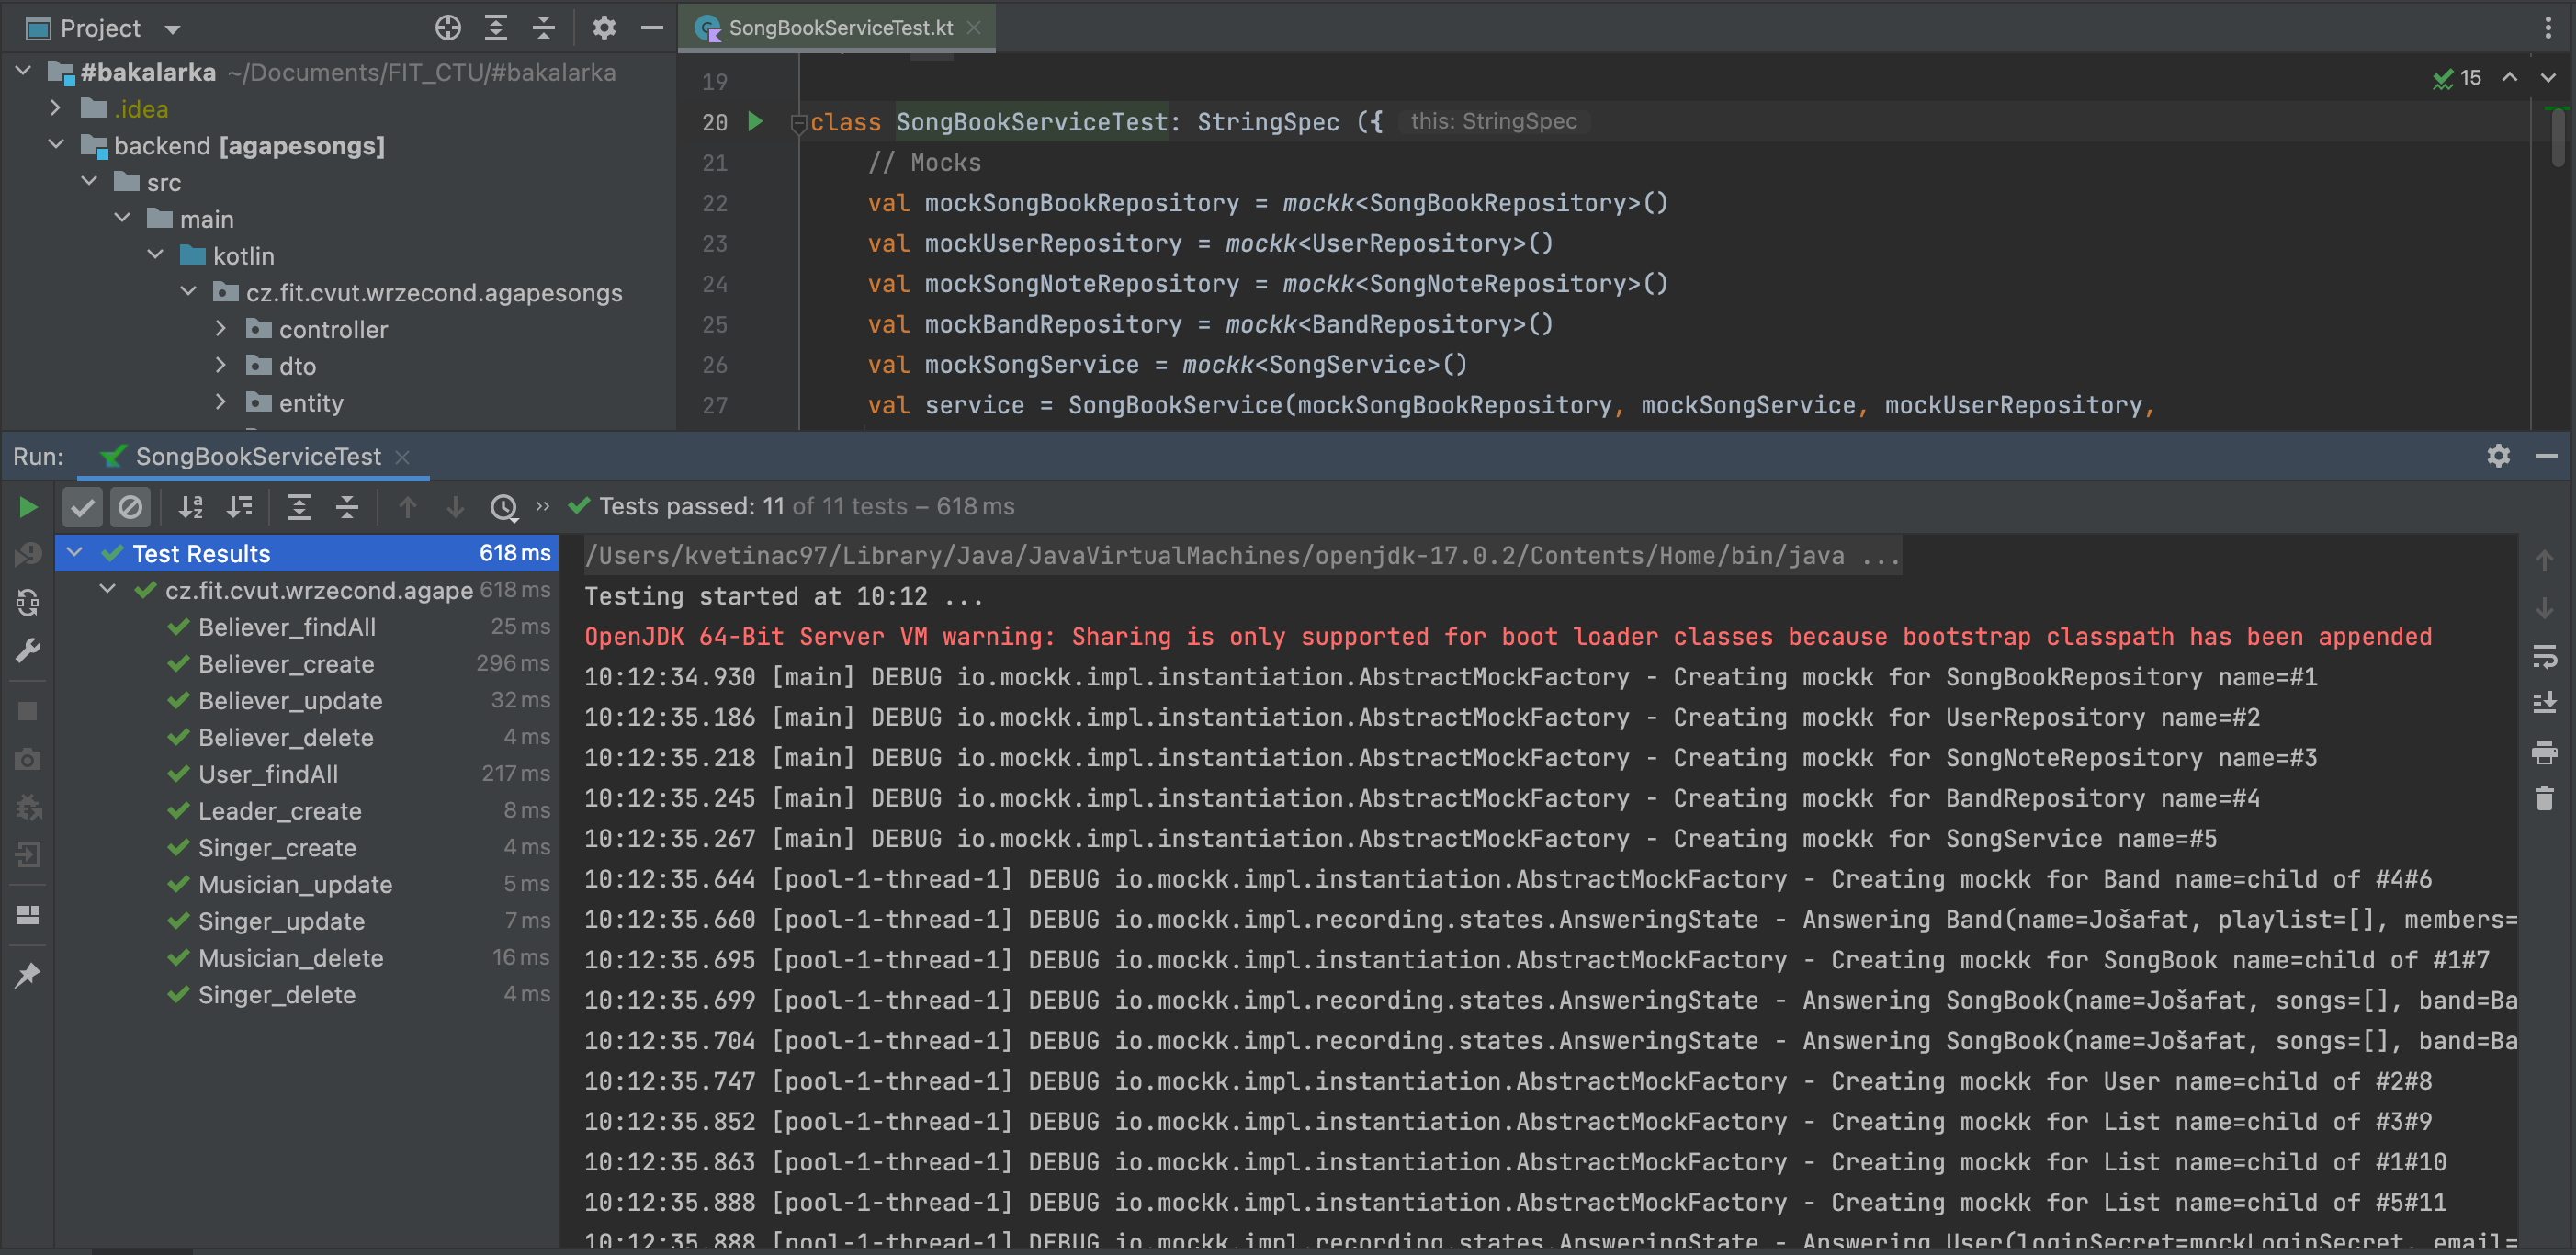
\includegraphics[width=\textwidth]{images/6-testovani/6-1-unit-test-server.png}
    \caption{Ukázka úspěšně provedených jednotkových testů serveru}
\end{figure}

\subsubsection{Aplikace}

Pro testování mobilní aplikace jsem využil nativní framework XCTest \cite{xctest}. V tomto frameworku každá třída dědí ze třídy \texttt{XCTestCase} a jednotlivé testy jsou implementovány jako její metody. Před spuštěním každého testu je zavolána metoda \texttt{setUp()}, po jeho dokončení pak metoda \texttt{tearDown()}. Pro vytváření mocků nepoužívám žádný framework -- vytvářím je ručně pomocí protocol-oriented programování. Všechny testy v aplikaci pak dědí ze třídy \texttt{AgapeSongsTestCase}, do které jsem předpřipravil dependency injection mocků a třídy \texttt{AppState}.

\begin{listing}[H]
\begin{minted}[breaklines,breaksymbolleft=]{swift}
func testLoadSongBooksEmpty() async {
    songBookService.songBookListResponse = .success([SongBookDTO]())
    await viewModel.loadSongBooks()
    
    XCTAssertTrue(songBookService.songBookListCalled)
    XCTAssertEqual(viewModel.songBooks, [SongBook]())
    XCTAssertEqual(viewModel.state, .success)
}
\end{minted}
\caption[Ukázka metody pro otestování načtení seznamu zpěvníků v aplikaci]{Ukázka metody pro otestování načtení seznamu zpěvníků. Při testování je nejprve mocku nastavena odpověď, následně se asynchronně zavolá testovaná metoda a nakonec se zkontroluje, zda byla metoda zavolána a vrátila požadovanou návratovou hodnotu}
\end{listing}

\begin{figure}[H]
    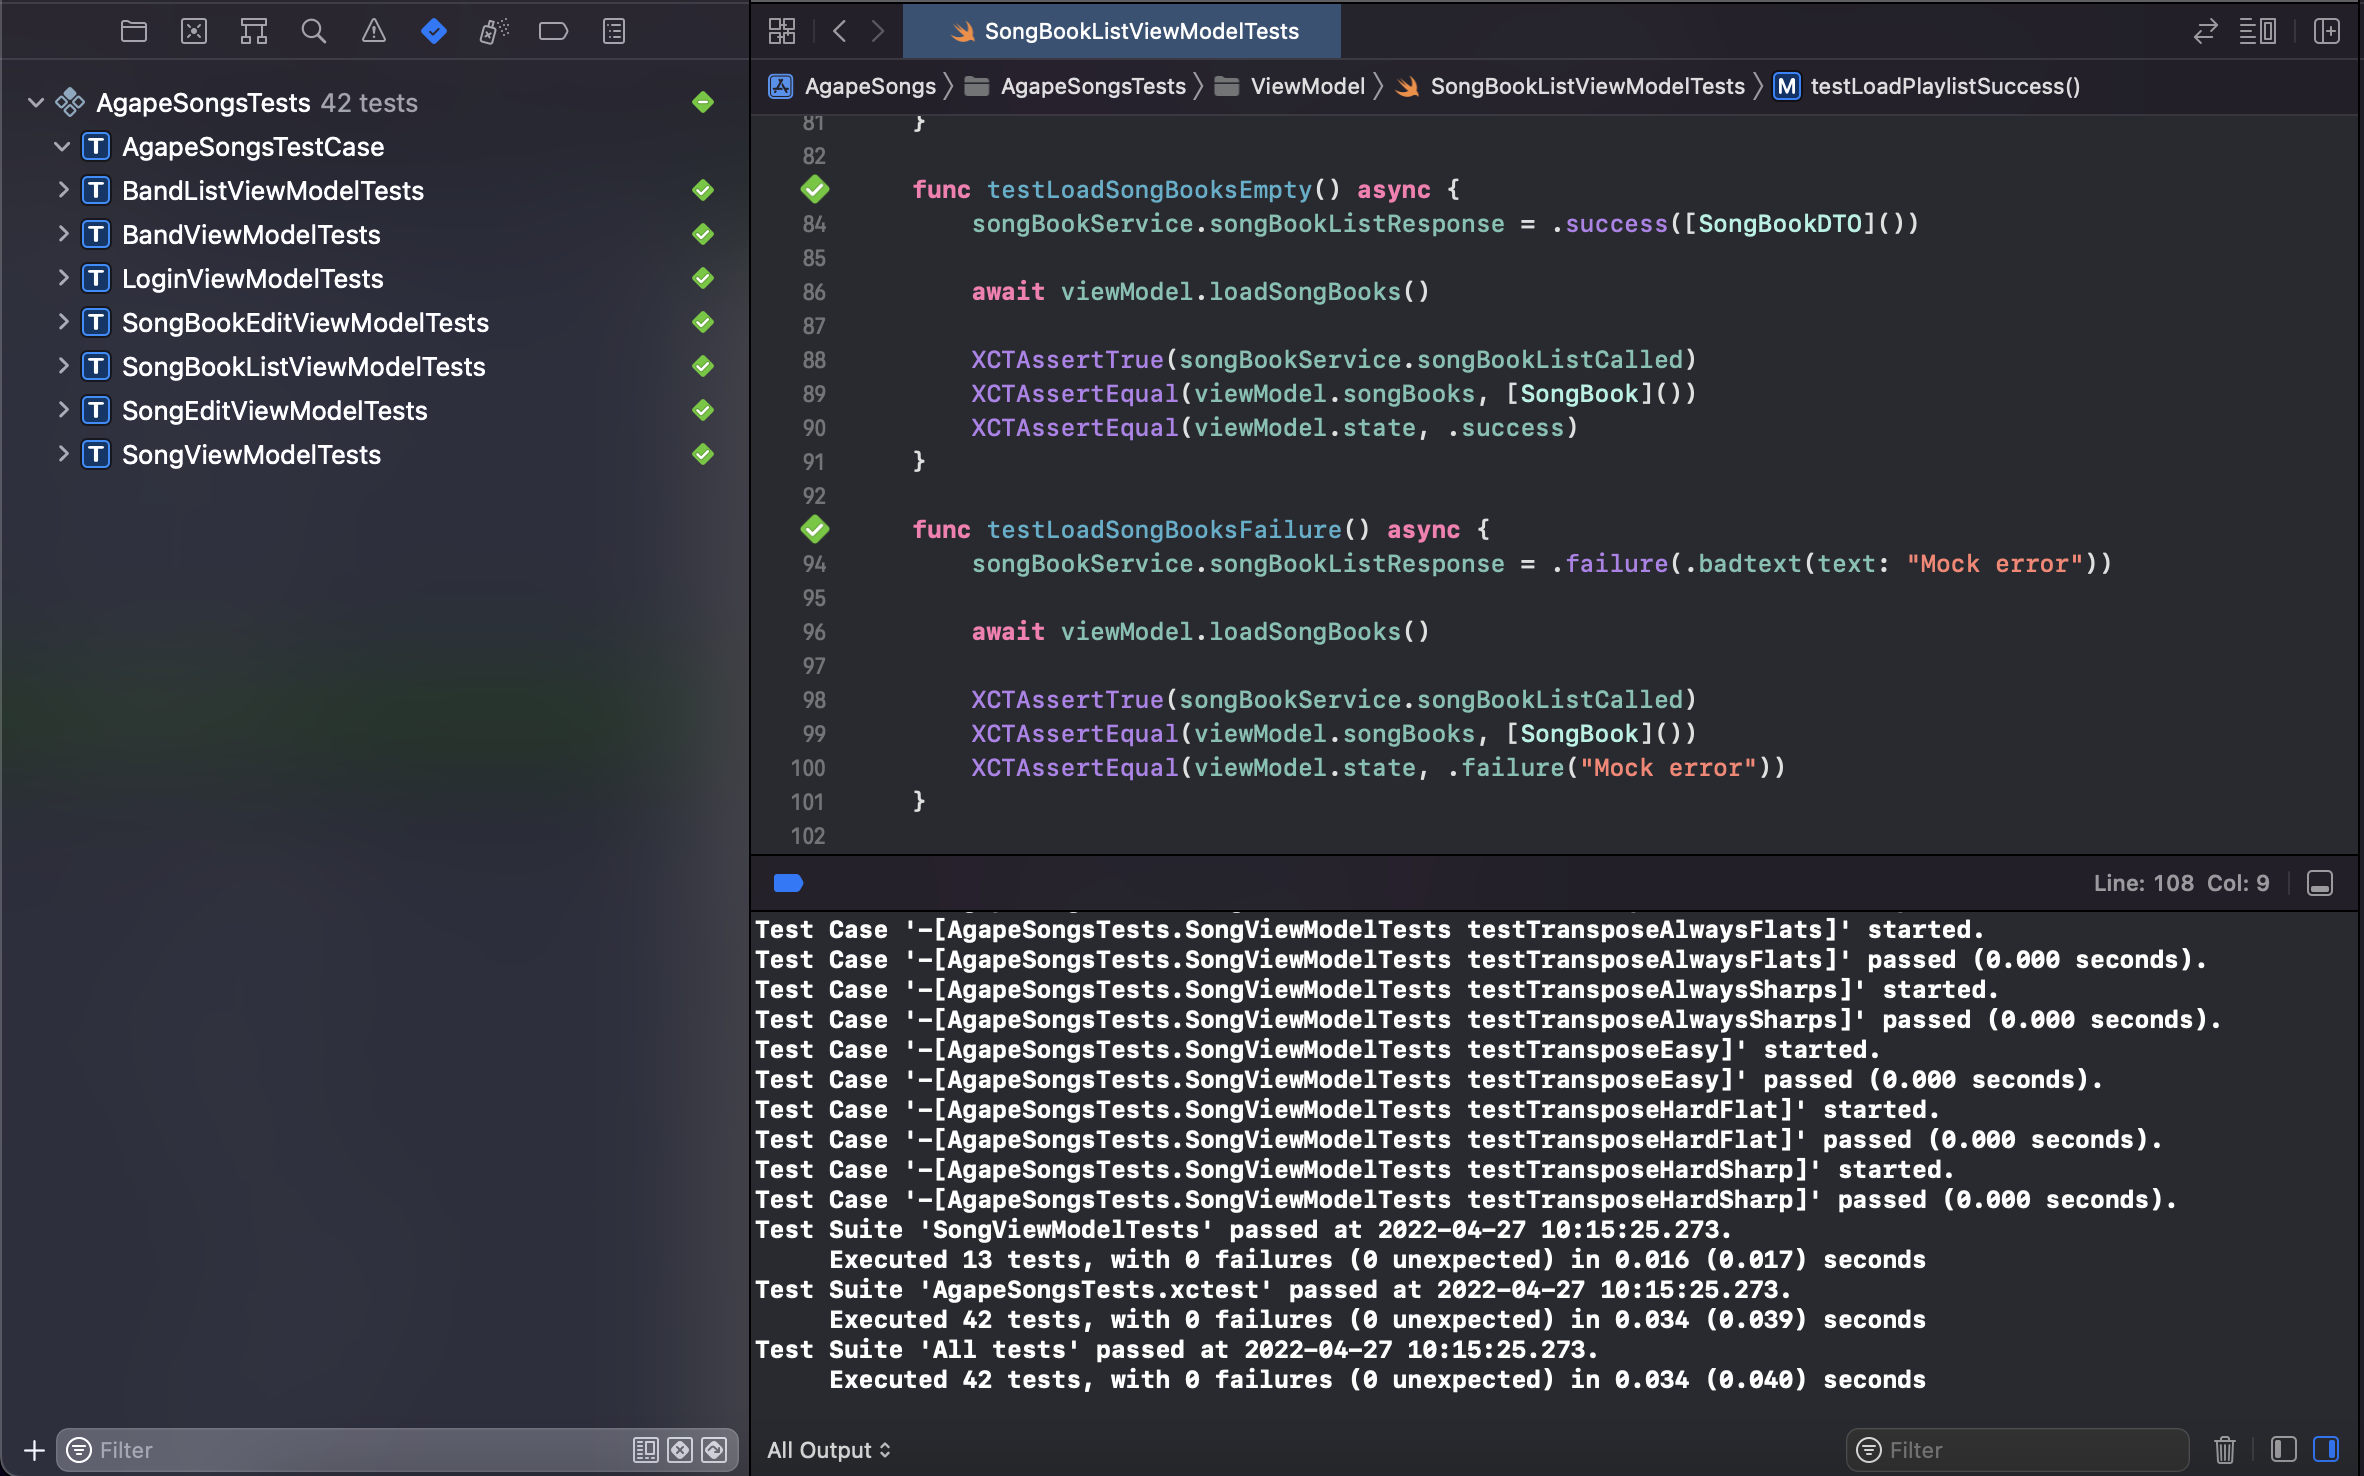
\includegraphics[width=\textwidth]{images/6-testovani/6-2-unit-test-aplikace.png}
    \caption{Ukázka úspěšně provedených jednotkových testů aplikace}
\end{figure}

\subsection{Integrační testy}

Automatizovaně testuji také vytvořené REST API, a to s pomocí programu Postman \cite{postman}. Ten umožňuje definovat jednotlivé sady požadavků a po provedení každého požadavku zavolat vlastní testy napsané v programovacím jazyce JavaScript.

\begin{listing}[H]
\begin{minted}[breaklines,breaksymbolleft=]{javascript}
pm.test("Response contains Agapebend first", function () {
    pm.expect(pm.response.json()[0].name).to.eql("Agapebend")
});
\end{minted}
\caption[Ukázka integračních testů v programu Postman]{Ukázka testu pro endpoint /songbook (zpěvníky), který zkontroluje, že odpověď na~požadavek je JSON pole, které obsahuje jeden zpěvník, jehož jméno je Agapebend}
\end{listing}

\begin{figure}[H]
    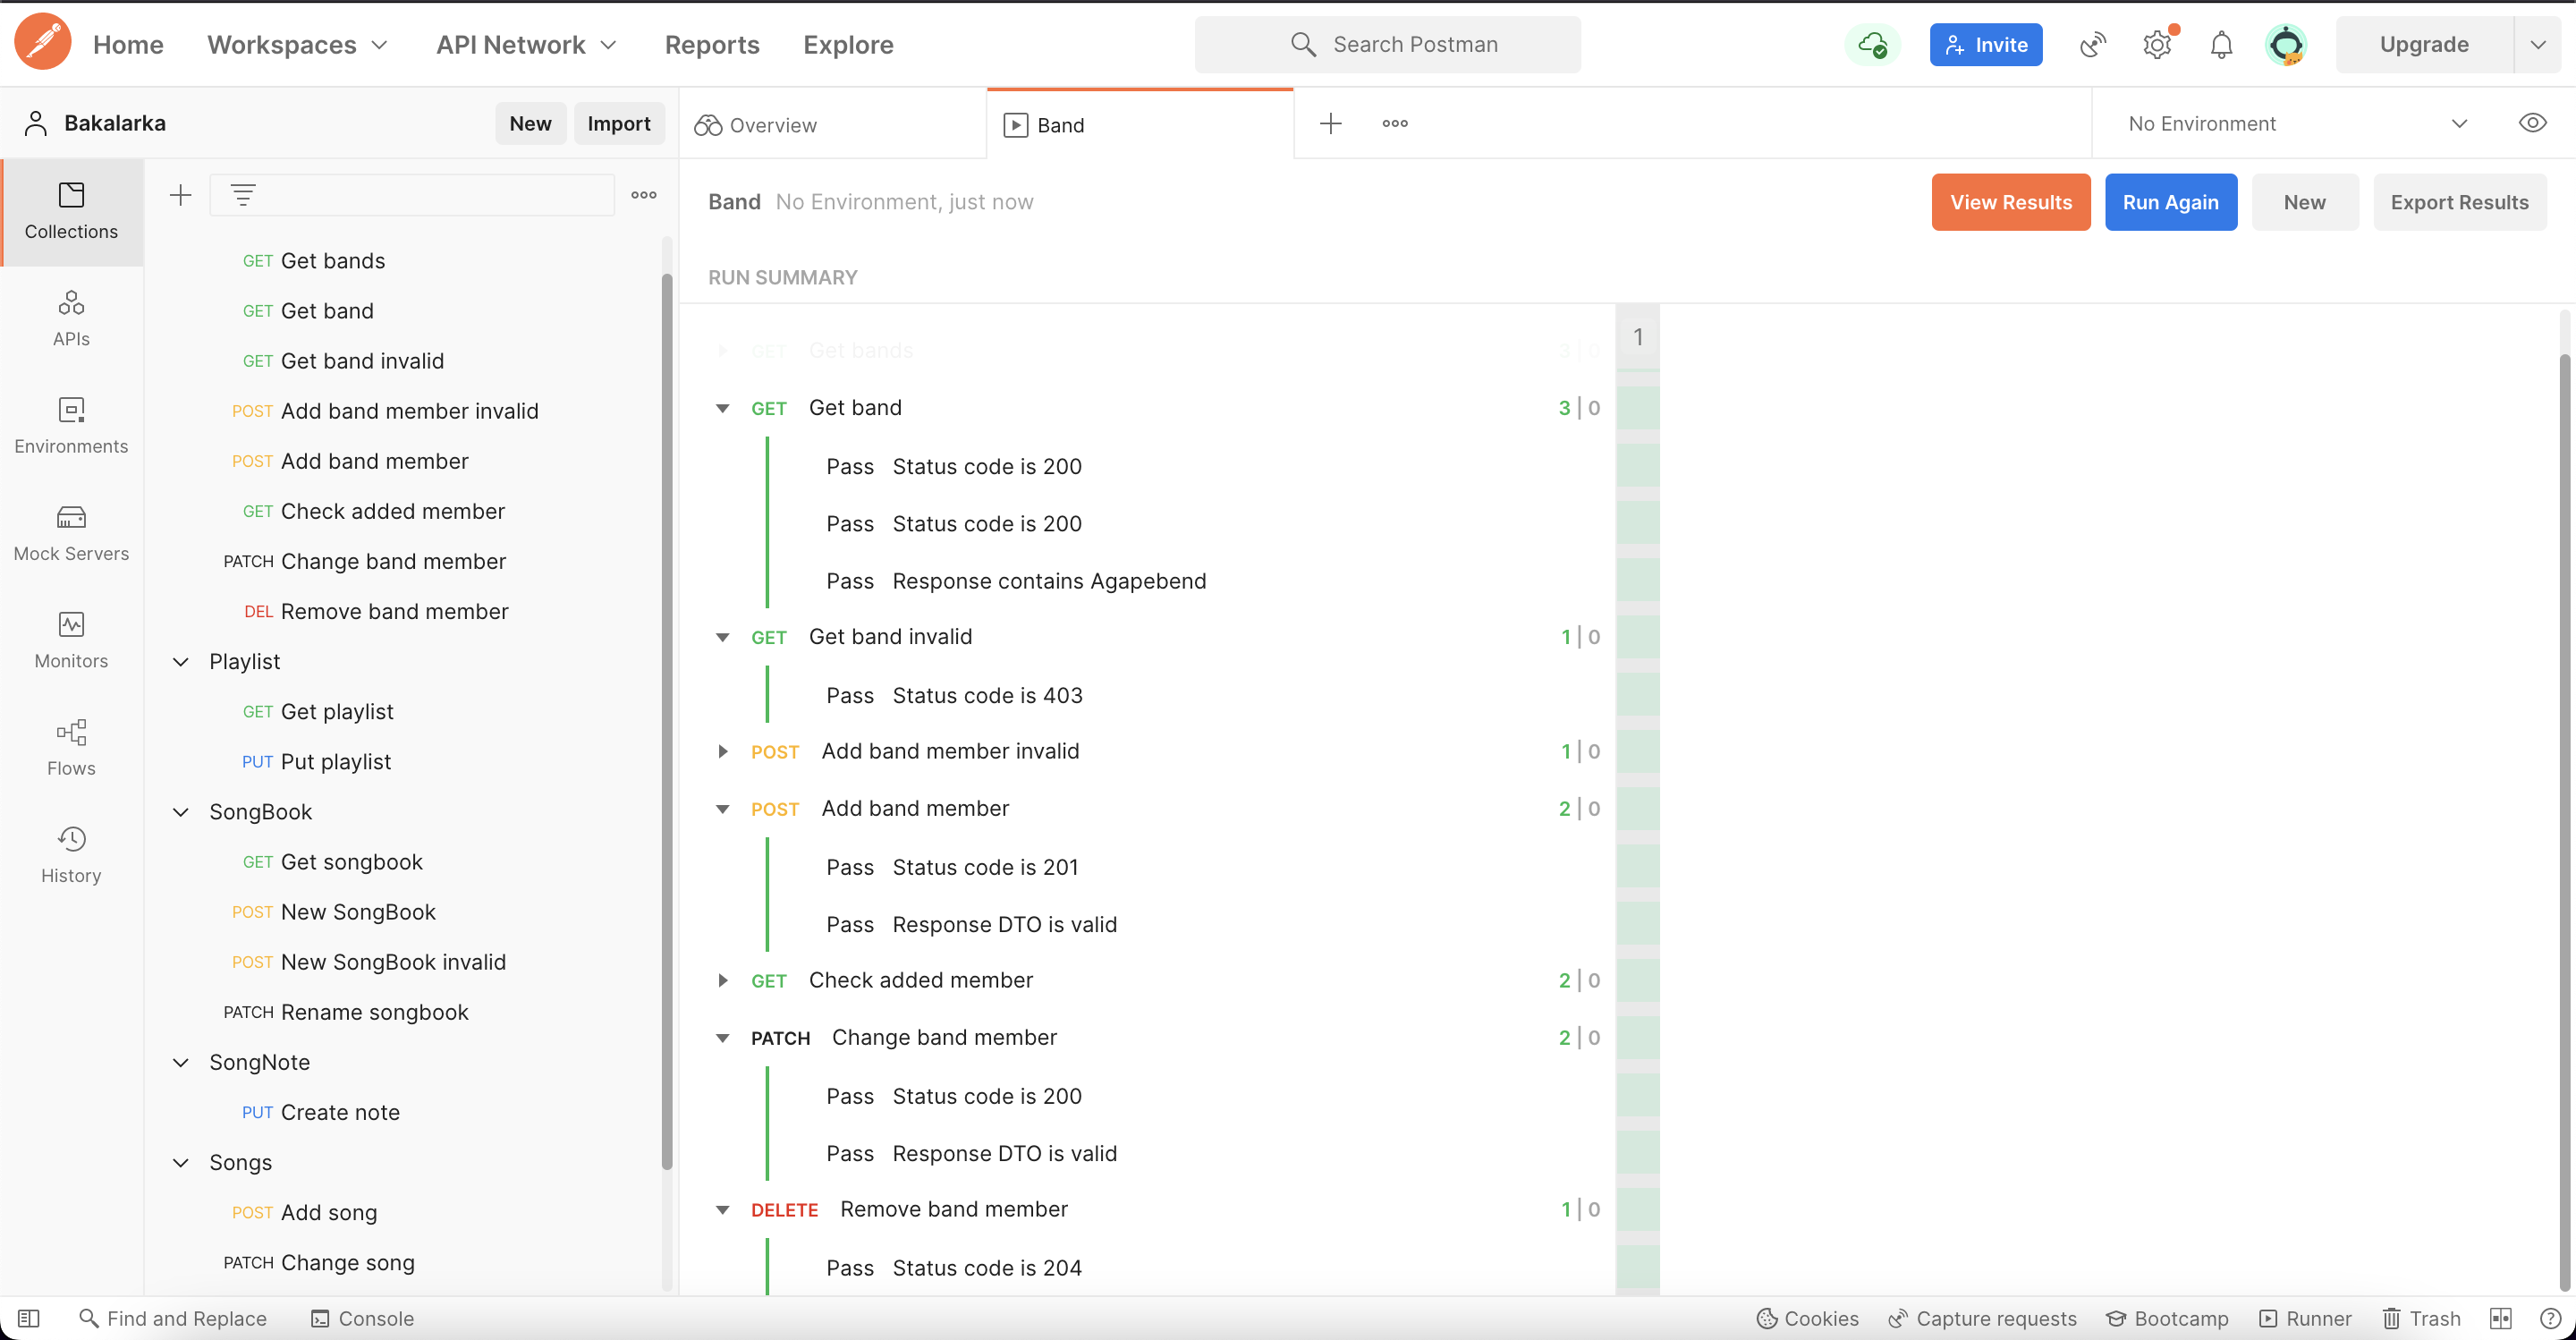
\includegraphics[width=\textwidth]{images/6-testovani/6-3-integracni-test-postman.png}
    \caption{Ukázka úspěšně provedených integračních testů pro endpoint /band}
\end{figure}

\subsection{Přínos}

Díky jednotkovým testům jsem byl schopen v serveru nebo v aplikaci chybu odhalit ještě dříve, než jsem je předal uživatelům k testování. Jednalo se například o chybu na serveru, kdy u písně, která již měla nastavené číslo v rámci zpěvníku nešlo toto číslo odstranit nebo chybu, kdy se při změně písně na začátek textu vždy přidal nový řádek. V aplikaci jsem pomocí jednotkových testů odhalil chyby v logice pro zalamování a chybu, kdy jsem zapomněl přidat možnost tóniny A dur. S pomocí integračních testů API v programu Postman jsem odhalil chybu, kdy API poskytovalo seznam zpěvníků ve špatném pořadí.

\section{Uživatelské testy}

Uživatelské testy provádí přímo budoucí uživatelé systému. V průběhu uživatelských testů lze pozorovat způsob, jakým uživatelé systém používají a často odhalí chyby, na které programátoři v průběhu automatizovaných testů nepřišli. Dalším velkým přínosem uživatelských testů je pak také zpětná vazba na aktuální verzi aplikace.

\subsection{TestFlight}

Pro to, aby mohli uživatelé aplikaci testovat, je třeba, aby si aplikaci nainstalovali. Na Apple zařízení lze aplikaci oficiálně nainstalovat pouze ze dvou zdrojů -- oficiálního obchodu App Store \cite{app-store} a testovací platformy TestFlight \cite{testflight}. Zveřejnění v oficiálním obchodě ale není vhodnou metodou pro distribuci aplikace za účelem testování, protože takto zveřejněná aplikace je viditelná pro všechny uživatele iOS a macOS zařízení, což prozatím není žádoucí.

Testovací platforma TestFlight umožňuje přehlednou a jednoduchou správu a distribuci testovacích verzí aplikace. Nové verze se do ní nahrávají přímo z programovacího prostředí Xcode. Nahrané verze lze pak spravovat v prostředí App Store Connect \cite{app-store-connect}, odkud je lze distribuovat mezi dvě skupiny uživatelů -- interní a externí. Výhodou interního testování je možnost okamžité distribuce, nevýhodou je ale nutnost uživatele přidat přímo jako členy organizace FIT ČVUT, což z technických důvodů v mém případě není možné.

\begin{figure}[H]
    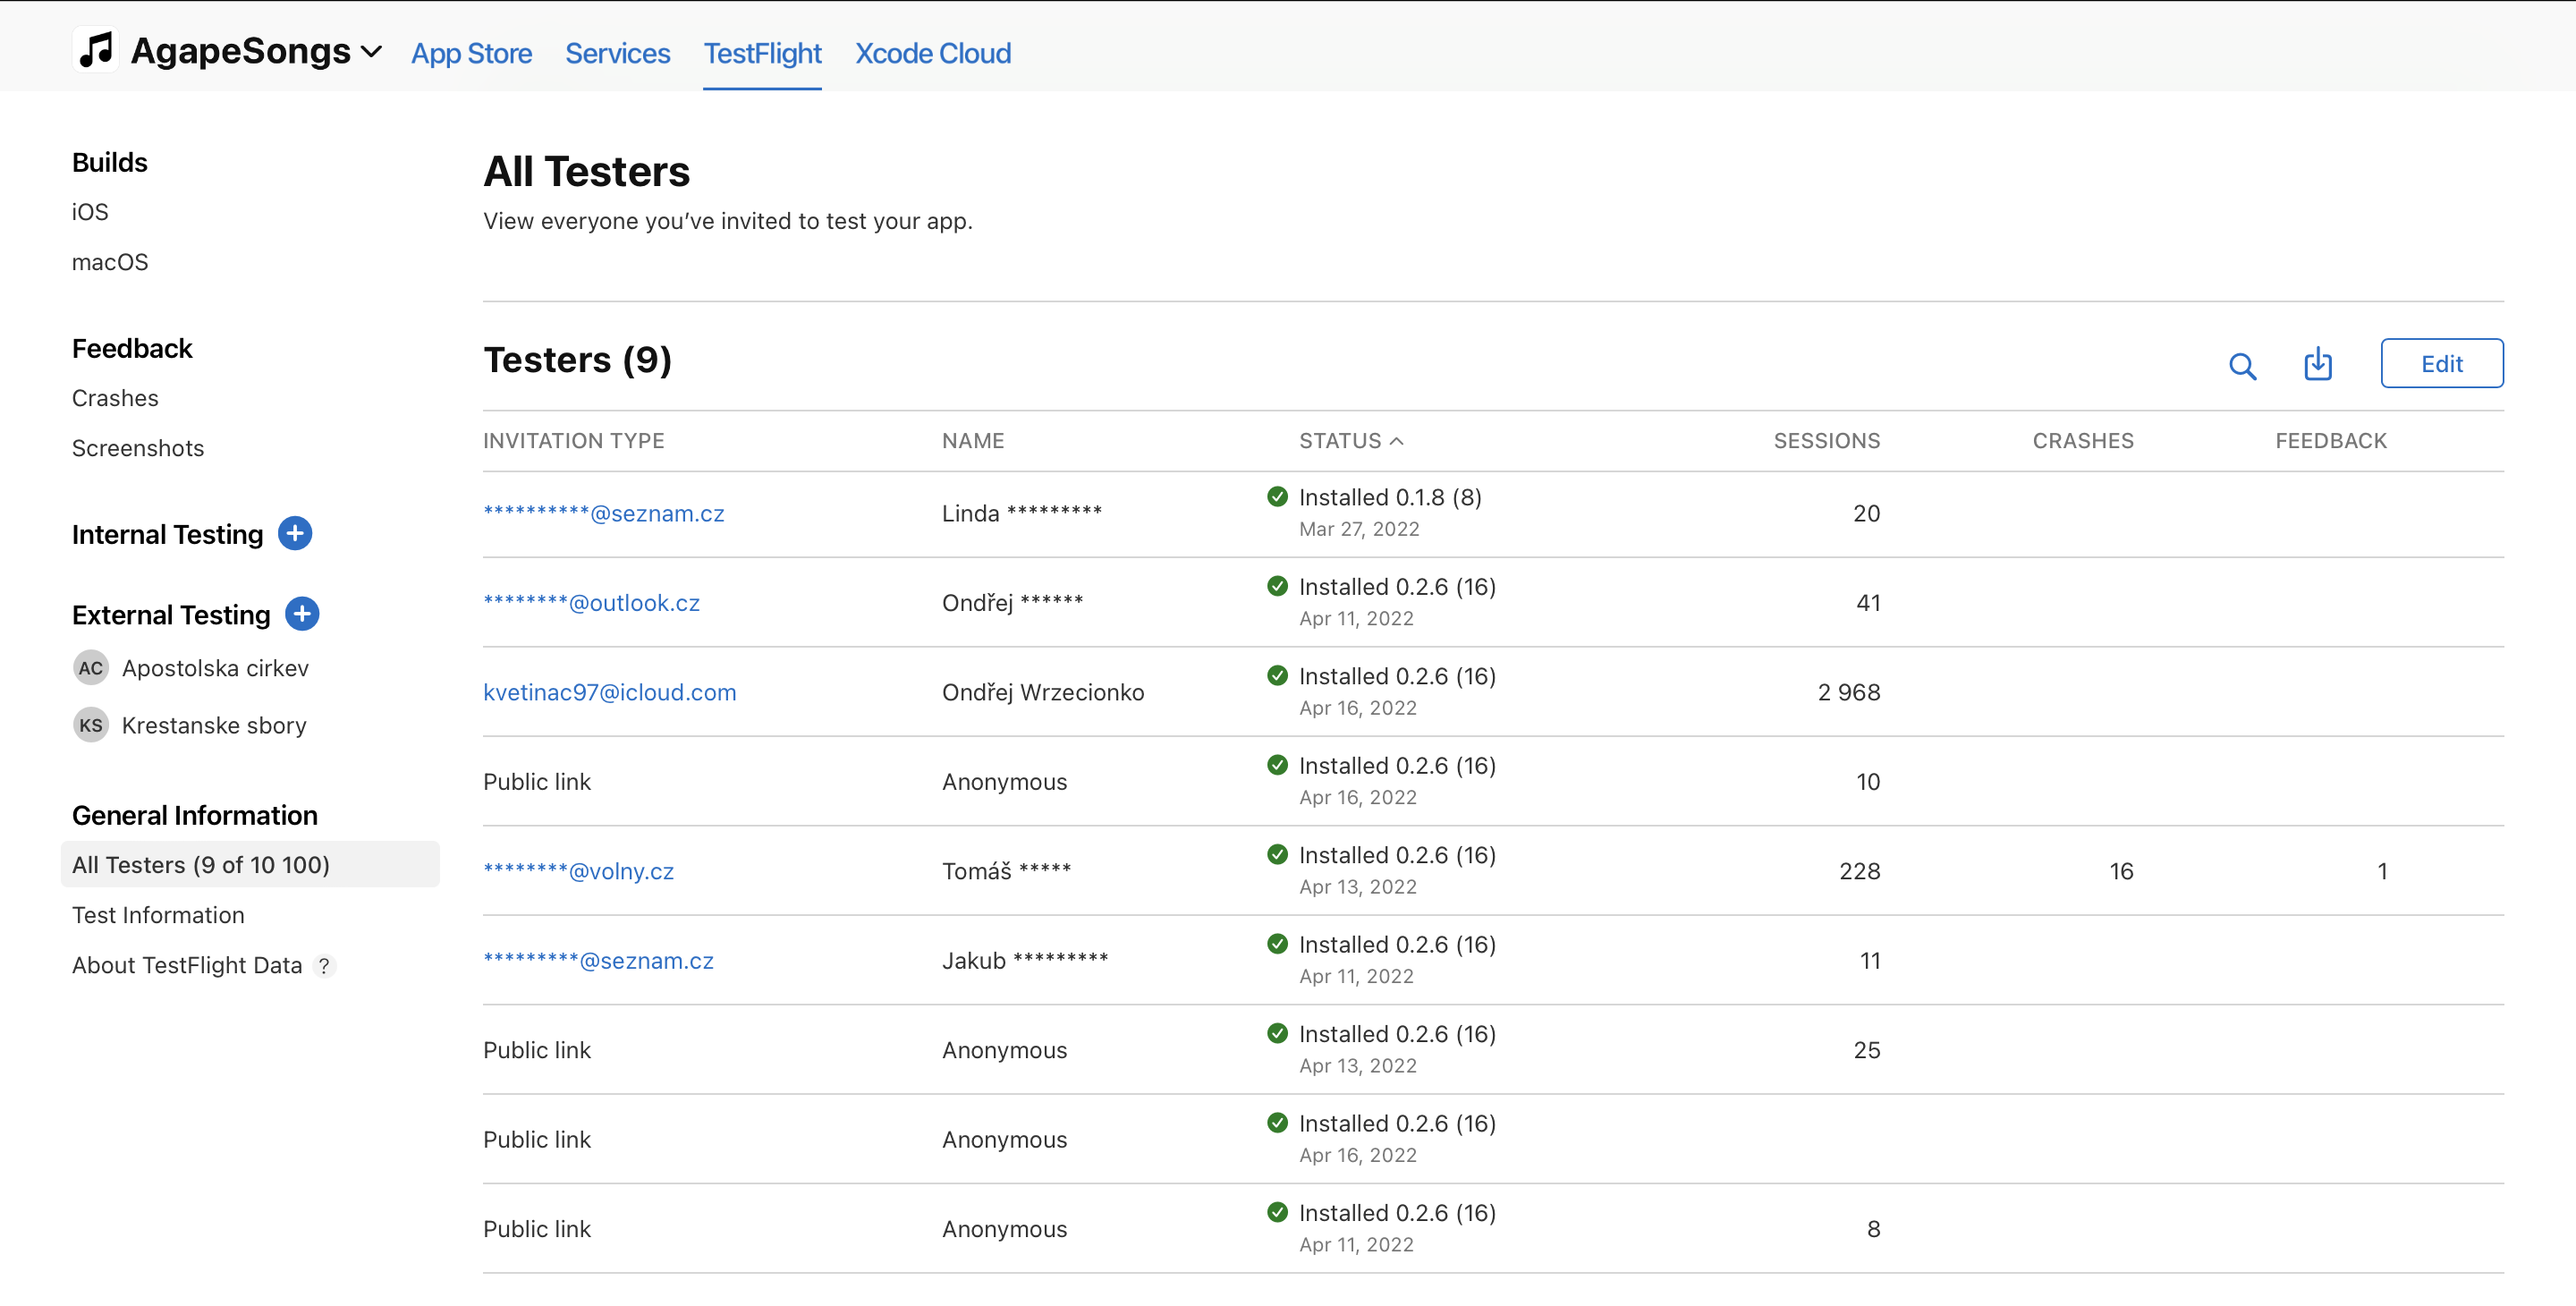
\includegraphics[width=\textwidth]{images/6-testovani/6-4-testflight-uzivatele.png}
    \caption{Ukázka správy testujících uživatelů v testovací platformě TestFlight}
\end{figure}

K externímu testování lze pozvat libovolného uživatele s Apple zařízením, nevýhodou je ale potřeba schválení každé nové verze ve zrychleném procesu App Review, který v praxi trvá přibližně 1 až 2 pracovní dny. Pro testování aplikace jsem si tedy vybral externí testování v rámci platformy TestFlight.

\begin{figure}[H]
    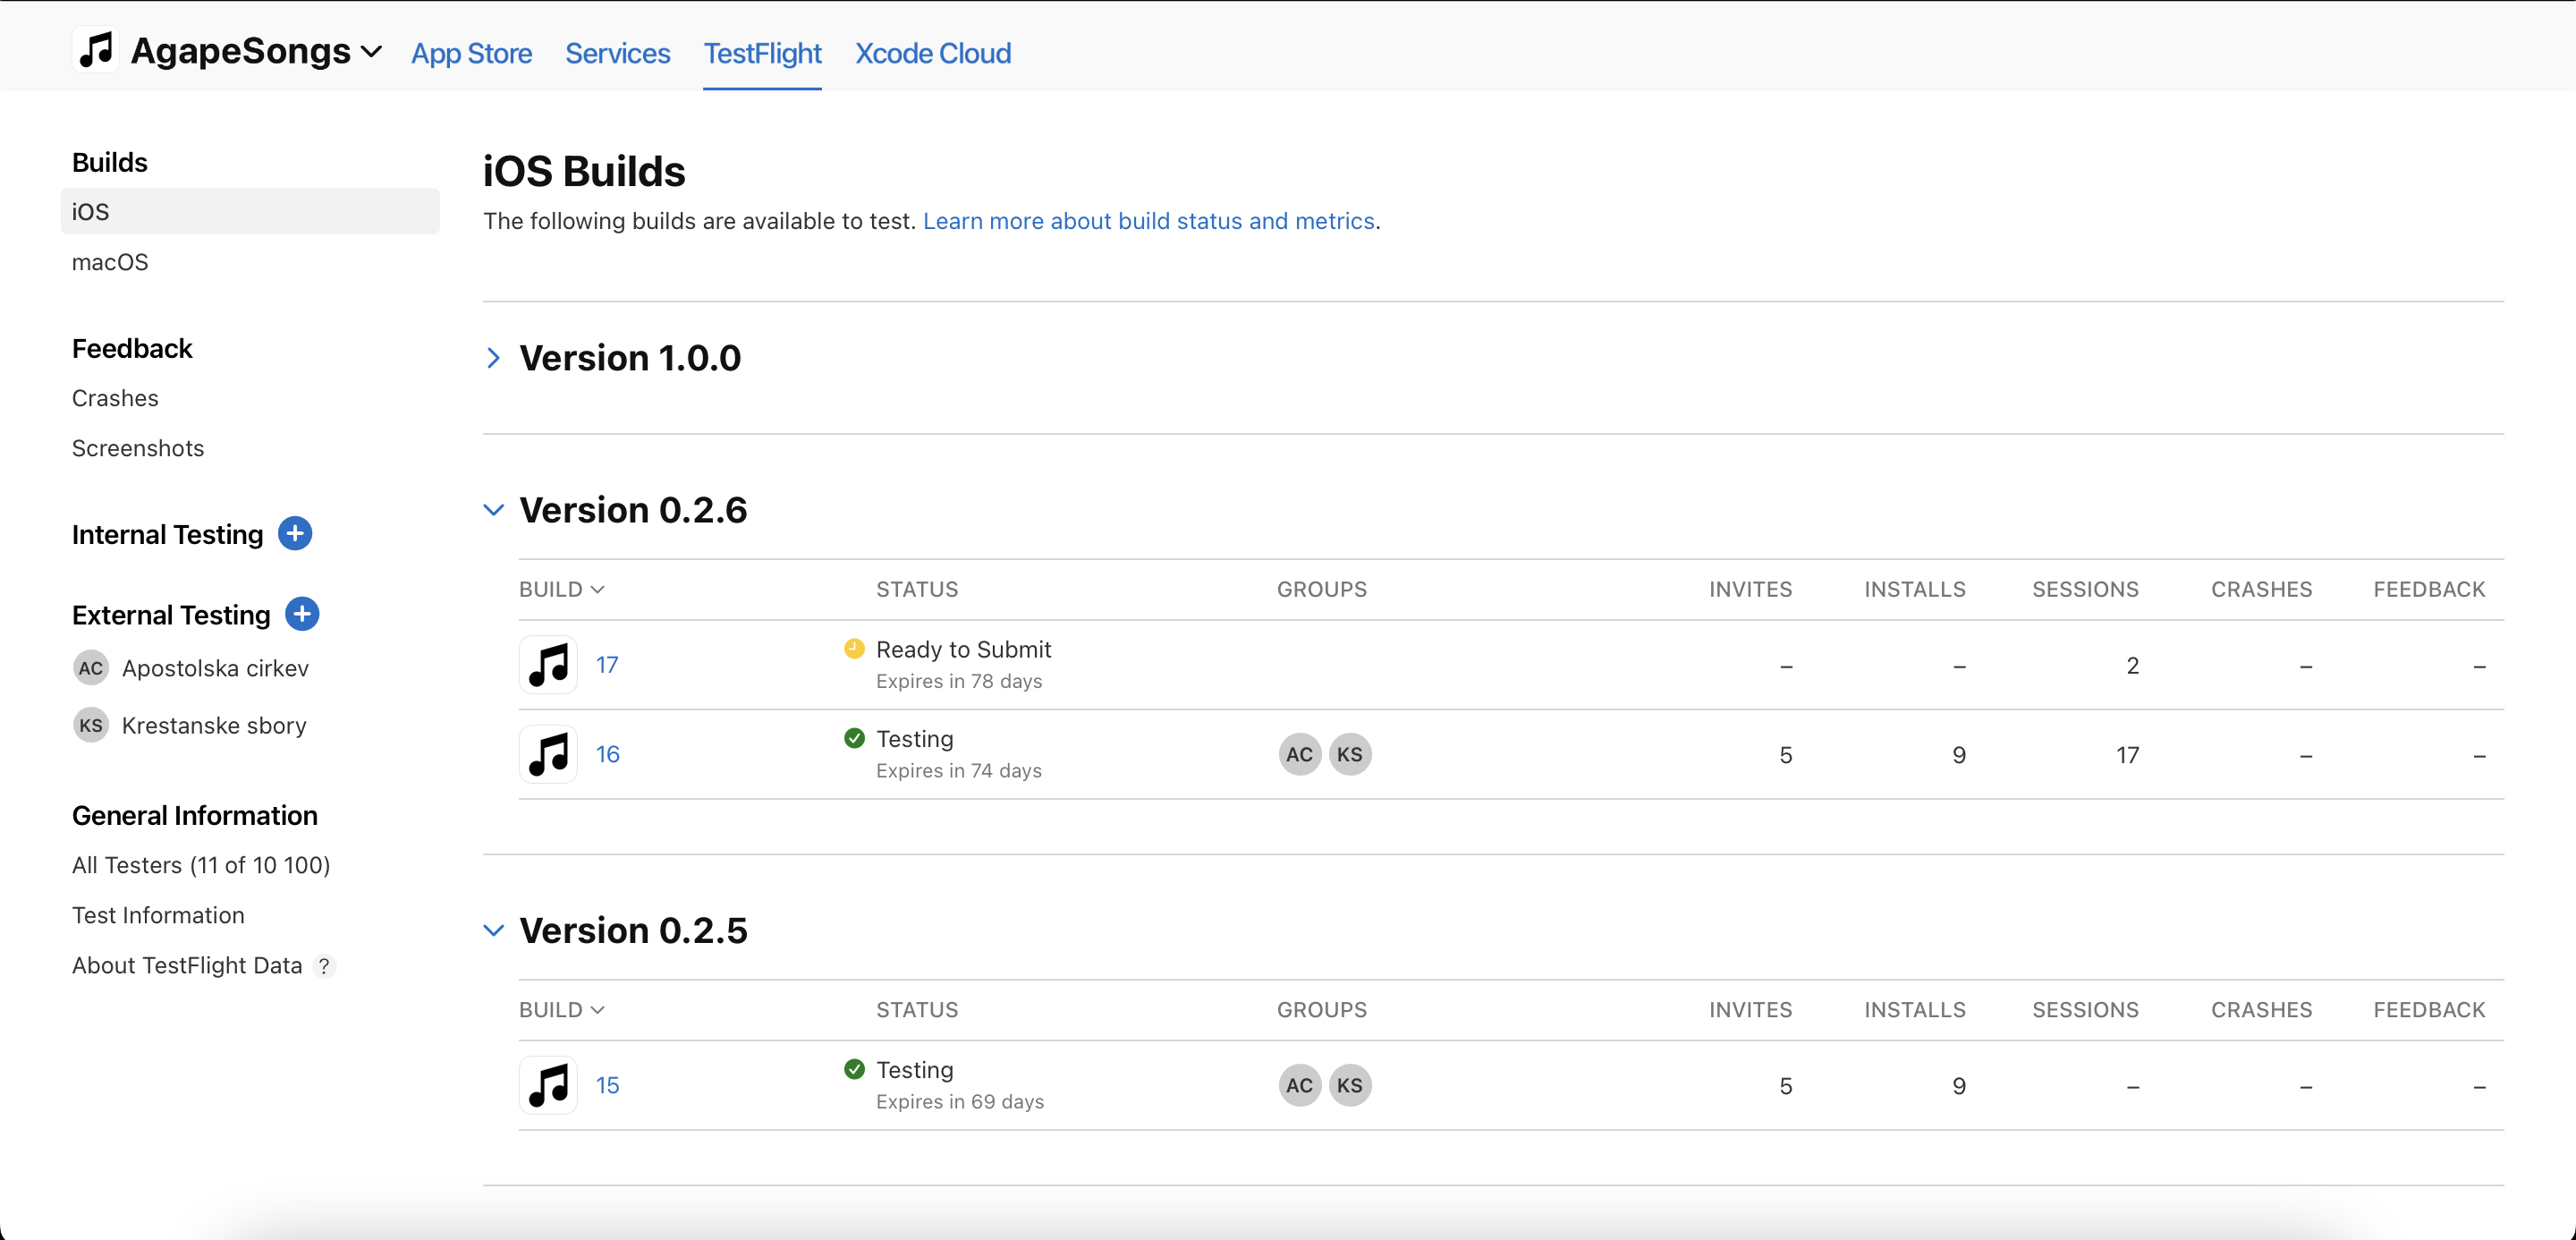
\includegraphics[width=\textwidth]{images/6-testovani/6-5-testflight-verze.png}
    \caption{Ukázka správy verzí aplikace v testovací platformě TestFlight}
\end{figure}

\subsection{AC Agapé}

Nejdéle jsem aplikaci testoval ve spolupráci s jednou z kapel v AC Agapé. Jak jsem psal v~analýze, v~AC Agapé jsou dvě kapely, které se střídají. Věděl jsem tedy, že tato kapela bude zkoušet 26. 3. 2022, 9. 4. 2022 a 23. 4. 2022, snažil jsem se tedy naplánovat tvorbu aplikace tak, abych byl schopen na první ze zmíněných sobot dodat použitelnou verzi aplikace.

\subsubsection{První zkouška}

Ve středu 23. 3. 2022 jsem do TestFlightu odeslal první verzi aplikace, ve čtvrtek 24. 3. 2022 byla schválena a odeslal jsem ji do kapely k testování. Vedoucí kapely mi ale vzápětí odpověděl, že členům kapely aplikace nejde nainstalovat. Po pár minutách zkoumání jsme zjistili, že jsem aplikaci omylem nastavil minimální verzi podporovaného operačního systému jako iOS 15.4, respektive macOS 12.1, zatímco členové kapely mají na zařízeních starší verze. Okamžitě jsem tedy v aplikaci snížil minimální verzi na iOS 15.0 a macOS 12.0 a odeslal jí znova ke schválení. Apple jí ale schválil až v půlnoci ze soboty na neděli a první zkoušku jsem tedy promeškal. Ponaučil jsem se ale a věděl jsem tak, že další verzi musím členům kapely odeslat s minimálně týdenním předstihem.

\subsubsection{Druhá zkouška}

Verzi aplikace pro druhou zkoušku (v sobotu 9. 4. 2022) jsem nahrál do TestFlightu pro jistotu už 31. 3. 2022, tedy s více než týdenním předstihem. 1. 4. 2022 mi byla verze zamítnuta, jelikož obsahovala chráněný autorský obsah -- písně ve zpěvnících. Musel jsem tedy upravit server tak, aby nově registrovaným uživatelům zobrazil pouze ukázkový zpěvník s ukázkovou písní a skutečné písně zůstaly viditelné pouze pro stávající uživatele. Po této úpravě jsem aplikaci znovu odeslal ke~schválení a 3. 4. 2022 byla aplikace schválena. V průběhu týdne jsem pak ještě doimplementoval funkci transpozice akordů.

Na sobotní zkoušce kapely jsem pak byl přítomen jako pozorovatel a po zkoušce jsem s členy kapely diskutoval o tom, jak se jim aplikace používala. Hodně členů kapely si stěžovalo na malou velikost písma názvu písní v seznamu. Vedoucímu chybělo v názvu číslo písně ve zpěvníku, které sděloval členům kapely s papírovým zpěvníkem. Zásadnější chybou bylo pak nesprávné přizpůsobení aplikace světlému módu. Aplikace jsem totiž vyvíjel v tmavém módu s použitím bílé barvy textu, která na bílém pozadí nebyla vidět. Někteří členové kapely tak museli dočasně přepnout aplikaci do tmavého módu. Při používání transpozice si pak někteří členové stěžovali na formát akordů -- některým vadil formát s křížky, některým s béčky.

Na základě této zkoušky jsem k názvu písně v seznamu přidal její číslo a aplikaci jsem otestoval také ve světlém módu, přičemž jsem našel více míst, kde se zobrazoval bílý text na~bílém pozadí. Stížnosti ohledně velikosti písma a formátu akordů jsem vyřešil přidáním nové obrazovky Nastavení aplikace, ve které si může uživatel nastavit velikost textu v seznamech a preferovaný formát zobrazení akordů.

\begin{figure}
    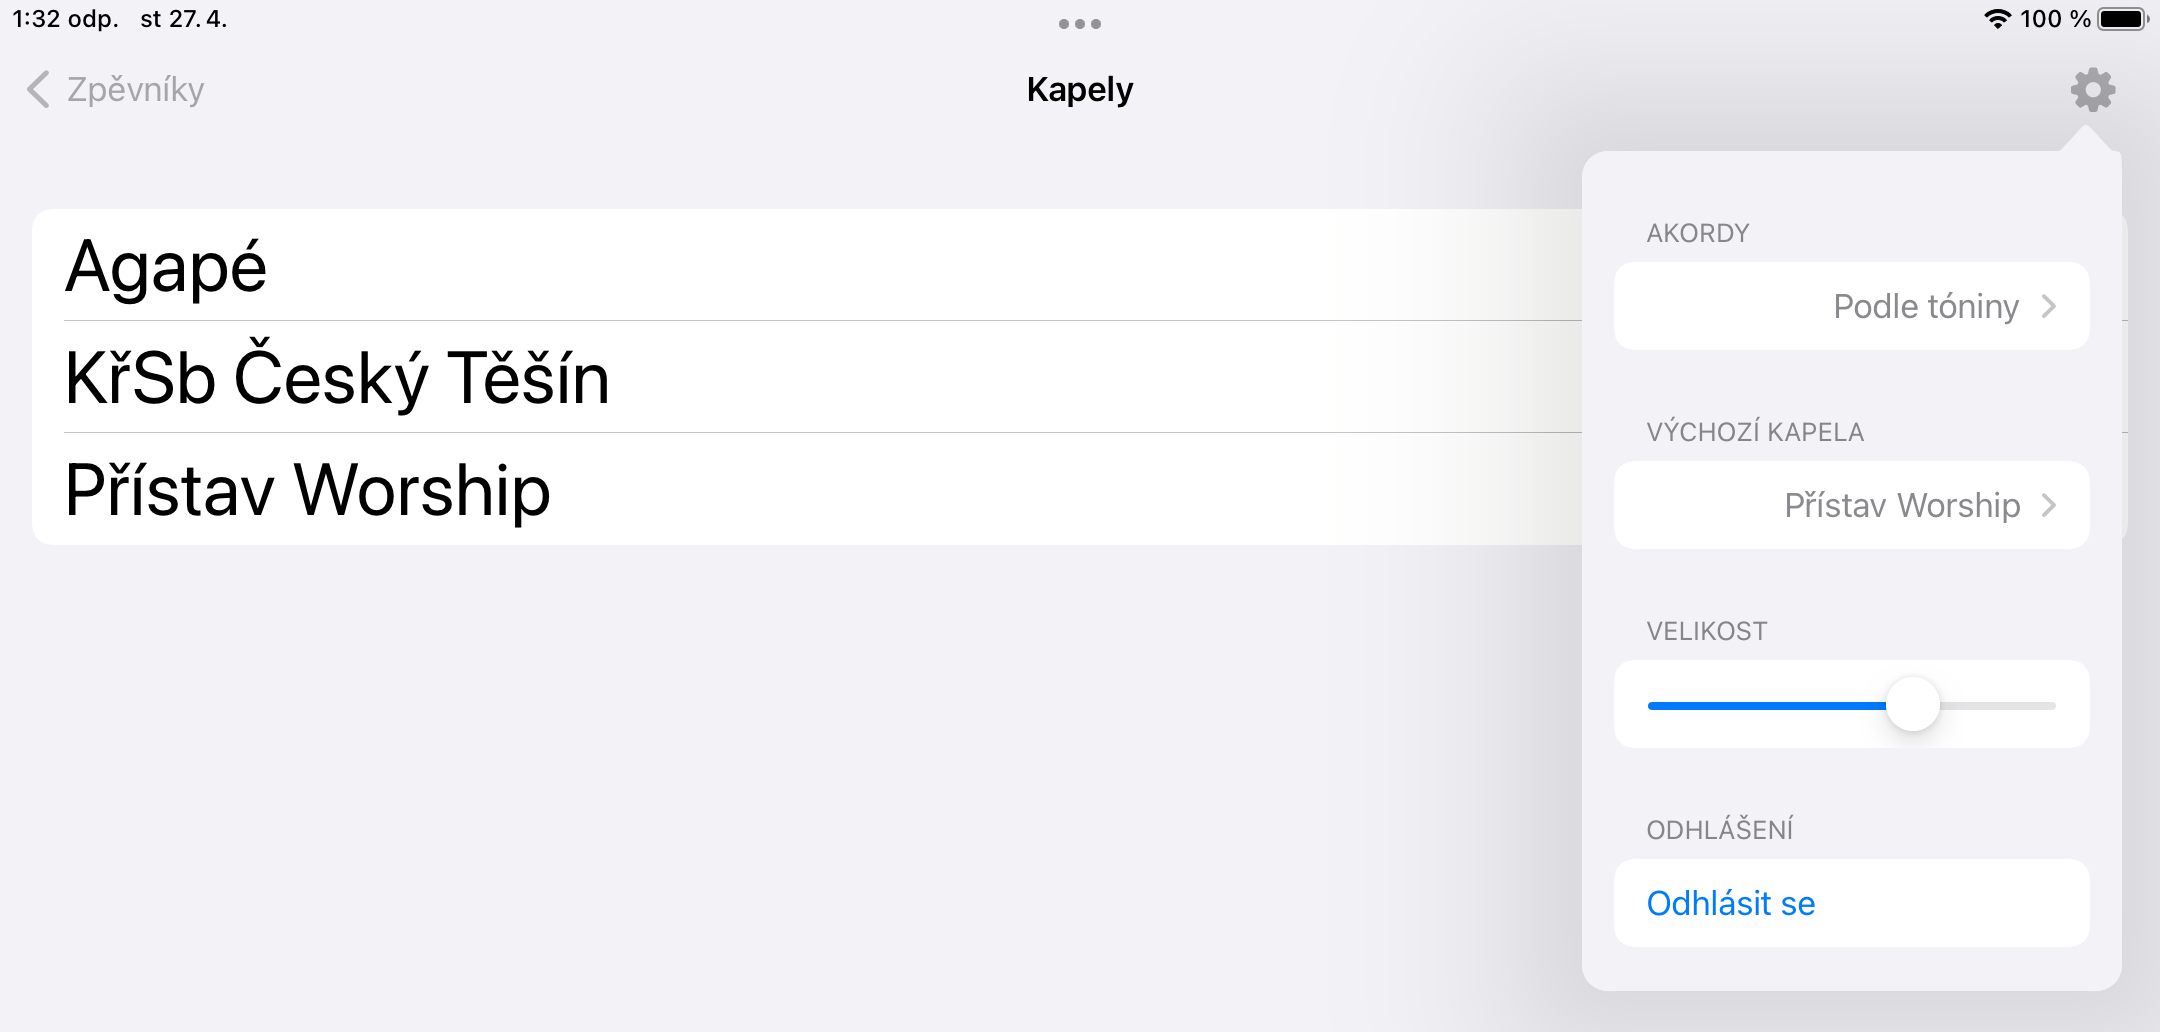
\includegraphics[width=\textwidth]{images/6-testovani/6-6-nastaveni-ipad.png}
    \caption[Ukázka obrazovky Nastavení aplikace na iOS]{Ukázka obrazovky pro nastavení velikosti písma, preferovaného formátu akordů a výchozí kapely pro nahrávání playlistu}
\end{figure}

\subsubsection{Třetí zkouška}

Třetí zkouška se konala v sobotu 23. 4. 2022. Po této zkoušce jsem dostal od členů kapely na~aplikaci již pouze pozitivní zpětnou vazbu spolu s návrhy na další vylepšení aplikace. Tyto návrhy podrobněji popíšu v kapitole \nameref{zaver}.

\subsection{Přístav Worship}

Další kapelou, ve které jsem testoval aplikaci, byla kapela Přístav Worship, která je součástí KřSb Český Těšín. Narozdíl od ostatních kapel je tato kapela složena převážně z mladých hudebníků, kteří všichni vlastní mobilní telefon s operačním systémem iOS. V rámci zkoušky Přístav Worship, která se konala v sobotu 16. 4. 2022, jsem tak měl možnost vyzkoušet také synchronizaci playlistů mezi více zařízeními v průběhu zkoušky.

Při zkoušce kapela našla dvě chyby -- první chybou byla nefunkční úprava písní, které jsou v~playlistu (po upravení písně v playlistu se text písně změnil až po jejím odebrání a znovupřidání do playlistu), což bylo v průběhu zkoušky zdržující a nepříjemné. Druhou, závažnější chybou pak byla situace, kdy se po nahrání a stažení v playlistu seřadily písně podle jejich unikátního identifikátoru a ne podle původního pořadí, což způsobilo mezi členy kapely zmatek.

Na základě této zkoušky jsem tedy zprovoznil úpravu písní v playlistu a také jsem opravil funkci pro nahrání a stahování playlistu na serveru tak, aby již neprováděla řazení playlistu podle unikátního identifikátoru.

\subsection{KřSb Pyšely}

Poslední kapelou, ve které jsem testoval aplikaci, byla kapela křesťanského sboru v Pyšelích, jejíž zkoušky jsem se účastnil o víkendu 23. - 24. dubna 2022. Zdejší kapela se skládá z tří hudebníků -- kytaristy a zpěvačky, kteří použili aplikaci na iPadu a klávesisty, který používal aplikaci na Macu. Kytarista a zpěvačka byli z aplikace nadšení a pouze předali návrhy dalších možných rozšíření aplikace. Klávesista při používání aplikaci našel chyby, které byly specifické pro používání aplikace na operačním systému macOS.

První chybou byla obtížnost používání aplikace spolu se softwarem MainStage, který klávesis\-té běžně používají pro hraní na klávesy. V průběhu hraní písně klávesista v této aplikaci, která se zobrazuje na celou obrazovku a nelze změnit její velikost, potřebuje přepínat rejstříky, zatímco se dívá na akordy v aplikaci. Aplikace by tedy v operačním systému macOS měla mít možnost zobrazení jako plovoucí okno.

\begin{figure}
    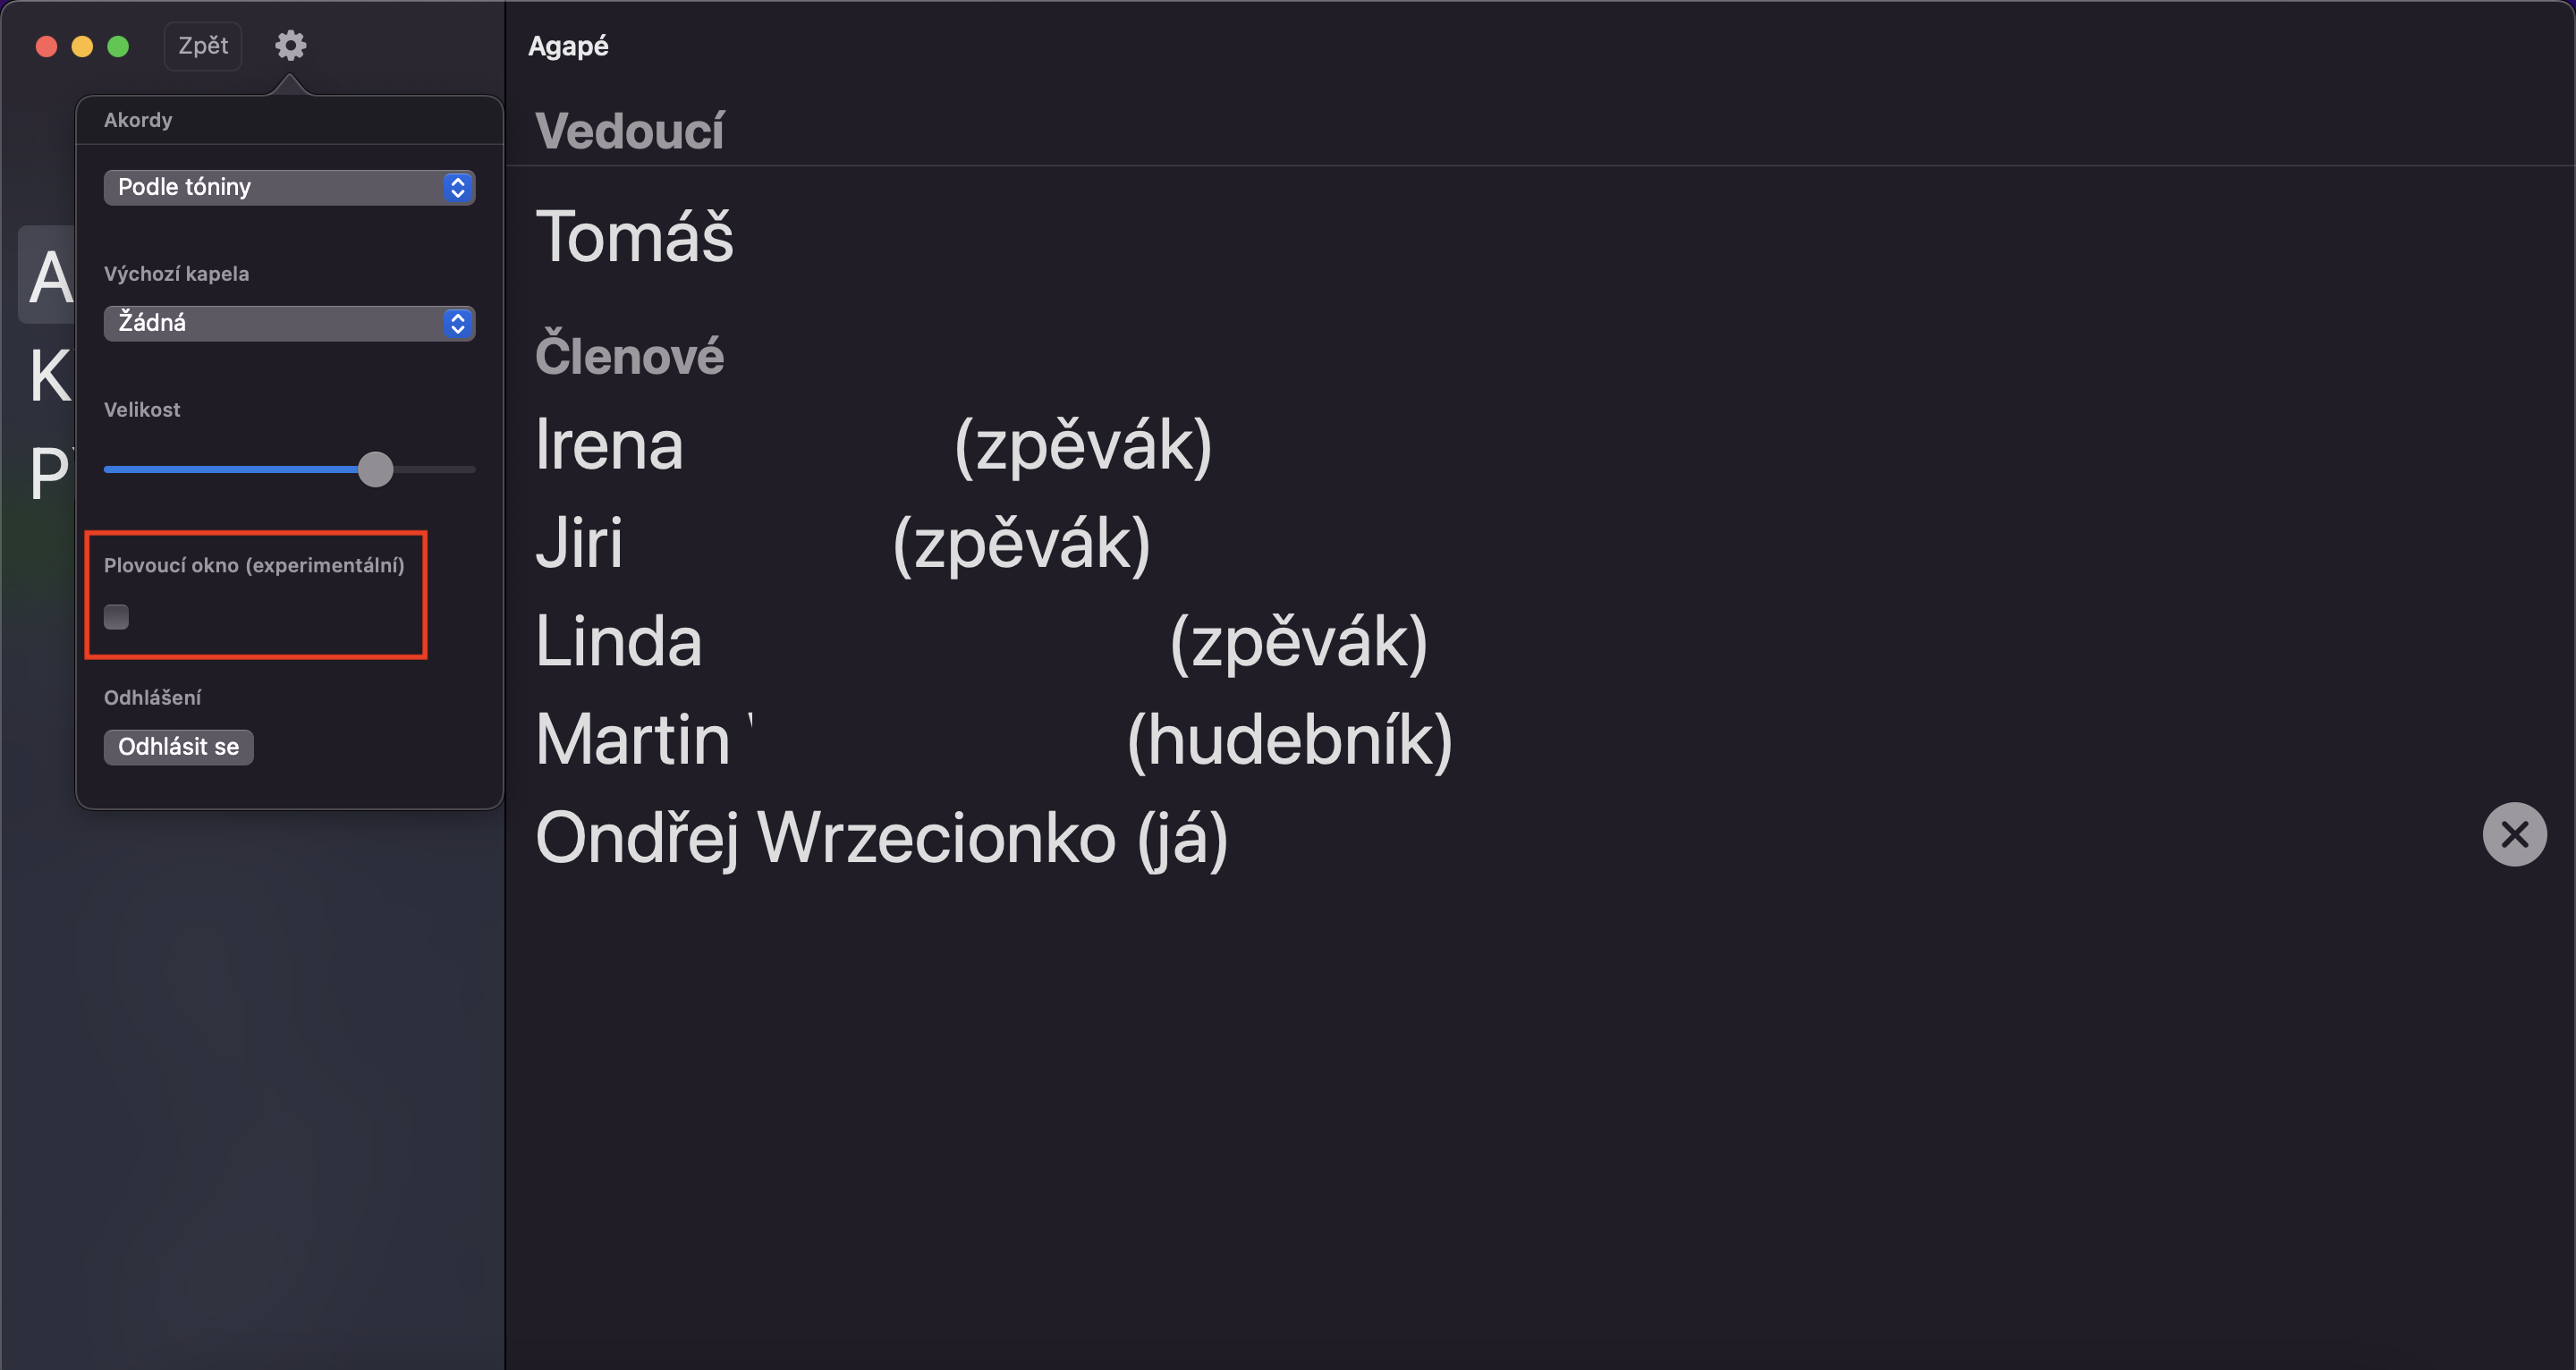
\includegraphics[width=\textwidth]{images/6-testovani/6-7-nastaveni-mac.png}
    \caption[Ukázka obrazovky Nastavení aplikace na macOS]{Nastavení režimu plovoucího okna v aplikaci na operačním systému macOS}
\end{figure}

Další chybou byla absence možnosti znovu načíst seznam písní přímo z aplikace. Po přidání nové písně tak ostatní členové kapely museli aplikaci ukončit a znovu spustit. Tyto chyby jsem vyřešil přidáním tlačítka pro zapnutí režimu plovoucího okna a tlačítka k znovu načtení seznamu písní.

\begin{figure}
    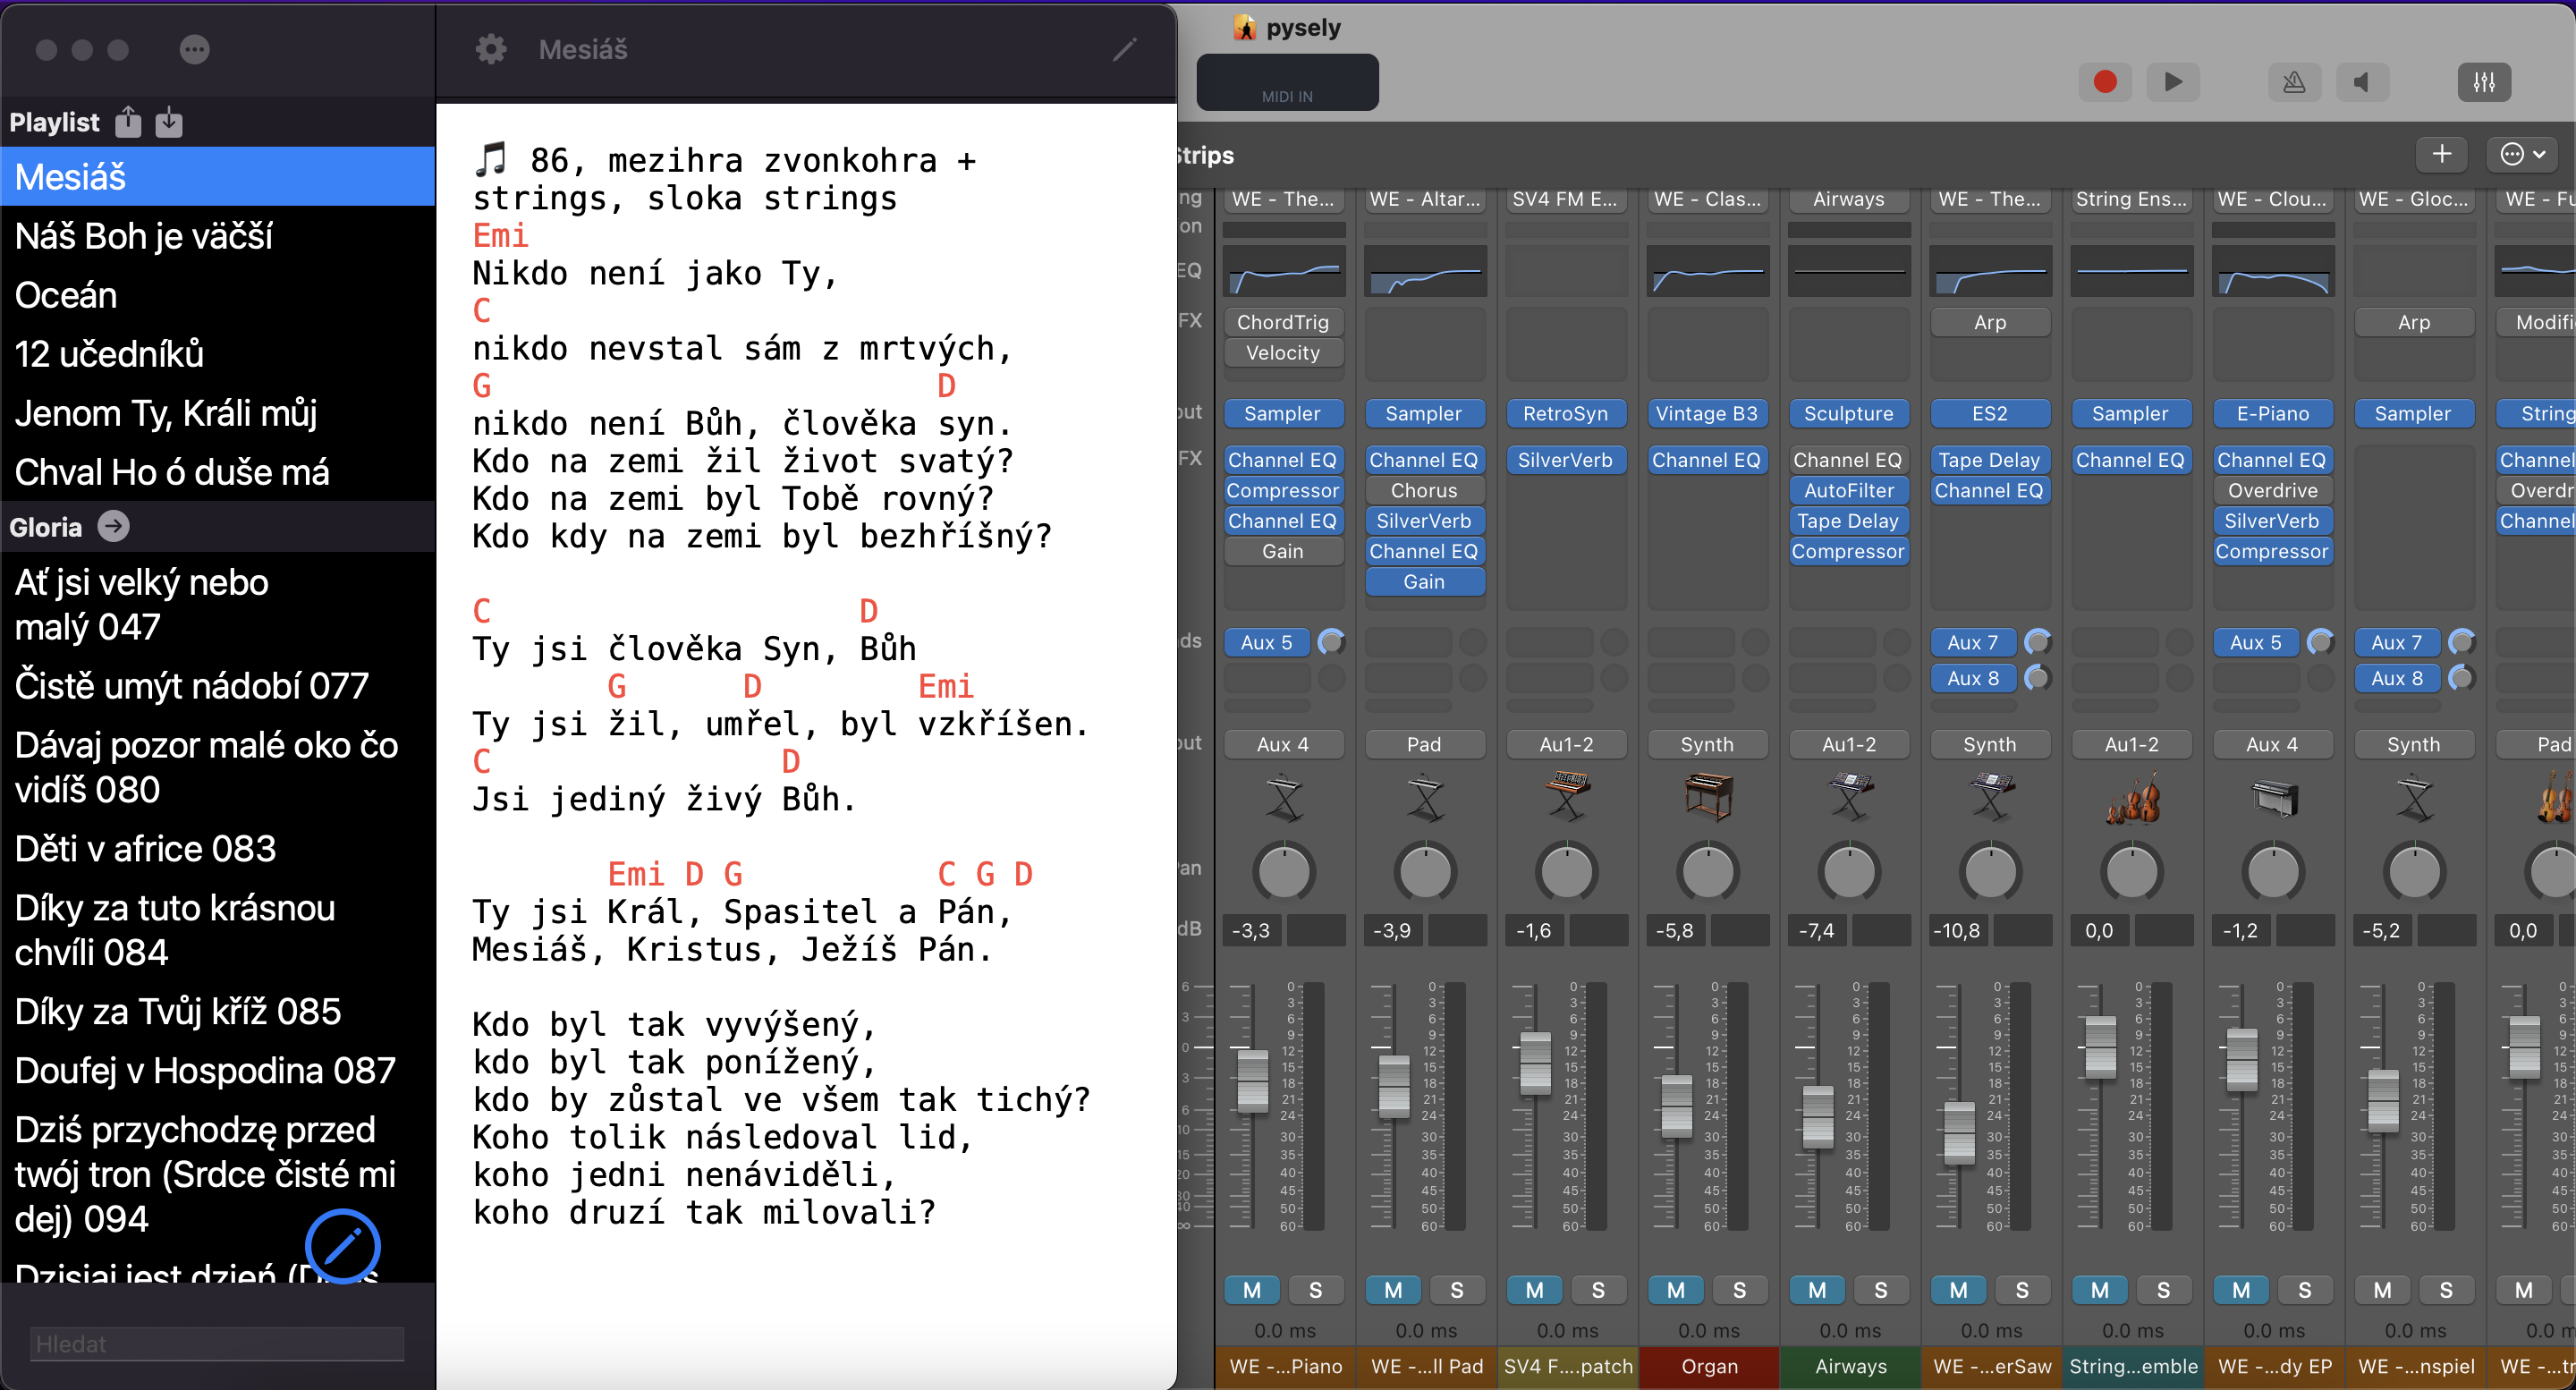
\includegraphics[width=\textwidth]{images/6-testovani/6-8-plovouci-okno.png}
    \caption{Zobrazení aplikace na macOS v režimu plovoucího okna}
\end{figure}

\subsection{Přínos}

V průběhu uživatelských testů jsem dostal mnoho zpětné vazby, díky které jsem mohl odhalit mnoho chyb v aplikaci, kterými byla absence čísla písně ve zpěvníku v názvu písně, nesprávné zobrazení některých komponent ve světlém módu, špatné nahrávání písní do playlistu nebo chybějící možnost znovu načtení seznamu písní. Dostal jsem také konkrétní návrhy na další funkcionality, které by členové hudebního doprovodu využili a které konkrétně popíšu v kapitole \nameref{zaver}.
